\section{Results (Block-by-Block Performance)}

\subsection{Block 1: Cohort Ingestion \& Feature Reduction Results}
We aggregate raw clinical and transcriptomic data from the Glioblastoma, Liver, Pancreatic, and Melanoma TCGA cohorts to assemble a base training matrix. We isolate the highest-variance $P_{\text{raw}} = 300$ genes [2] to mitigate the dimensionality curse inherent in multi-omic datasets. We execute an incremental Gram-Schmidt projection across these features to identify and discard collinear gene vectors with a cosine similarity threshold above $0.75$. Figure~\ref{fig:gram_schmidt_collinearity} displays the pairwise gene correlation heatmaps before and after applying this threshold. We standardize the remaining features via a $\log_2$ transformation to form the scaled matrix $Z_{\text{gene}} \in \mathbb{R}^{N \times 300}$. We extract latent variance structures by projecting this standardized matrix onto a right-singular eigenvector loading matrix $V \in \mathbb{R}^{300 \times 50}$ [1]. Figure~\ref{fig:pca_gene_loadings} illustrates this precise mapping of raw transcriptomic markers onto the computed principal components. This mathematical transformation yields the latent genomic feature matrix $X_{\text{pca}} \in \mathbb{R}^{N \times 50}$ [2]. We compile a standardized clinical feature matrix $X_{\text{clin}} \in \mathbb{R}^{N \times 9}$ comprising age, stage, sex, and tumor mutational burden. We concatenate these modalities to produce the unified model input feature matrix $X = [X_{\text{clin}} \mid X_{\text{pca}}] \in \mathbb{R}^{N \times 59}$. This dimensionality reduction strategy prevents Hessian matrix singularity during the optimization phases.

% -------------------------------------------------------------------------
% FIGURE 3: GRAM-SCHMIDT COLLINEARITY PRUNING HEATMAP (Side-by-Side)
% -------------------------------------------------------------------------
\begin{figure}[t]
    \centering
    \begin{minipage}{0.48\linewidth}
        \centering
        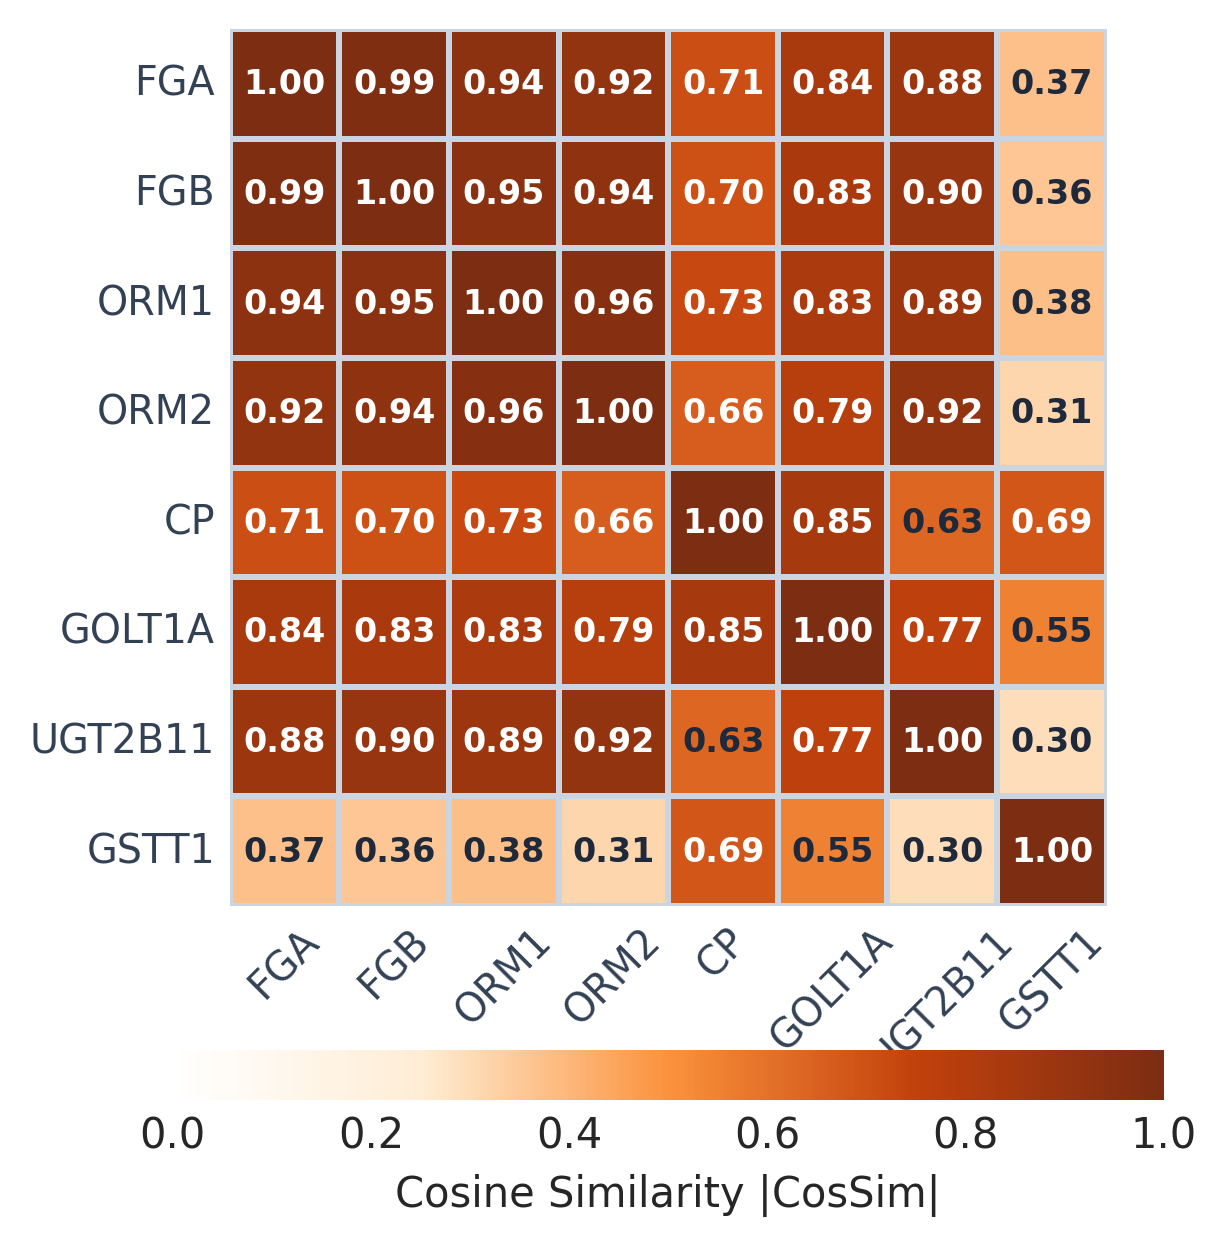
\includegraphics[width=\linewidth]{images/fig3a_collinearity_before.png}
        \subcaption{Before Projection}
    \end{minipage}\hfill
    \begin{minipage}{0.48\linewidth}
        \centering
        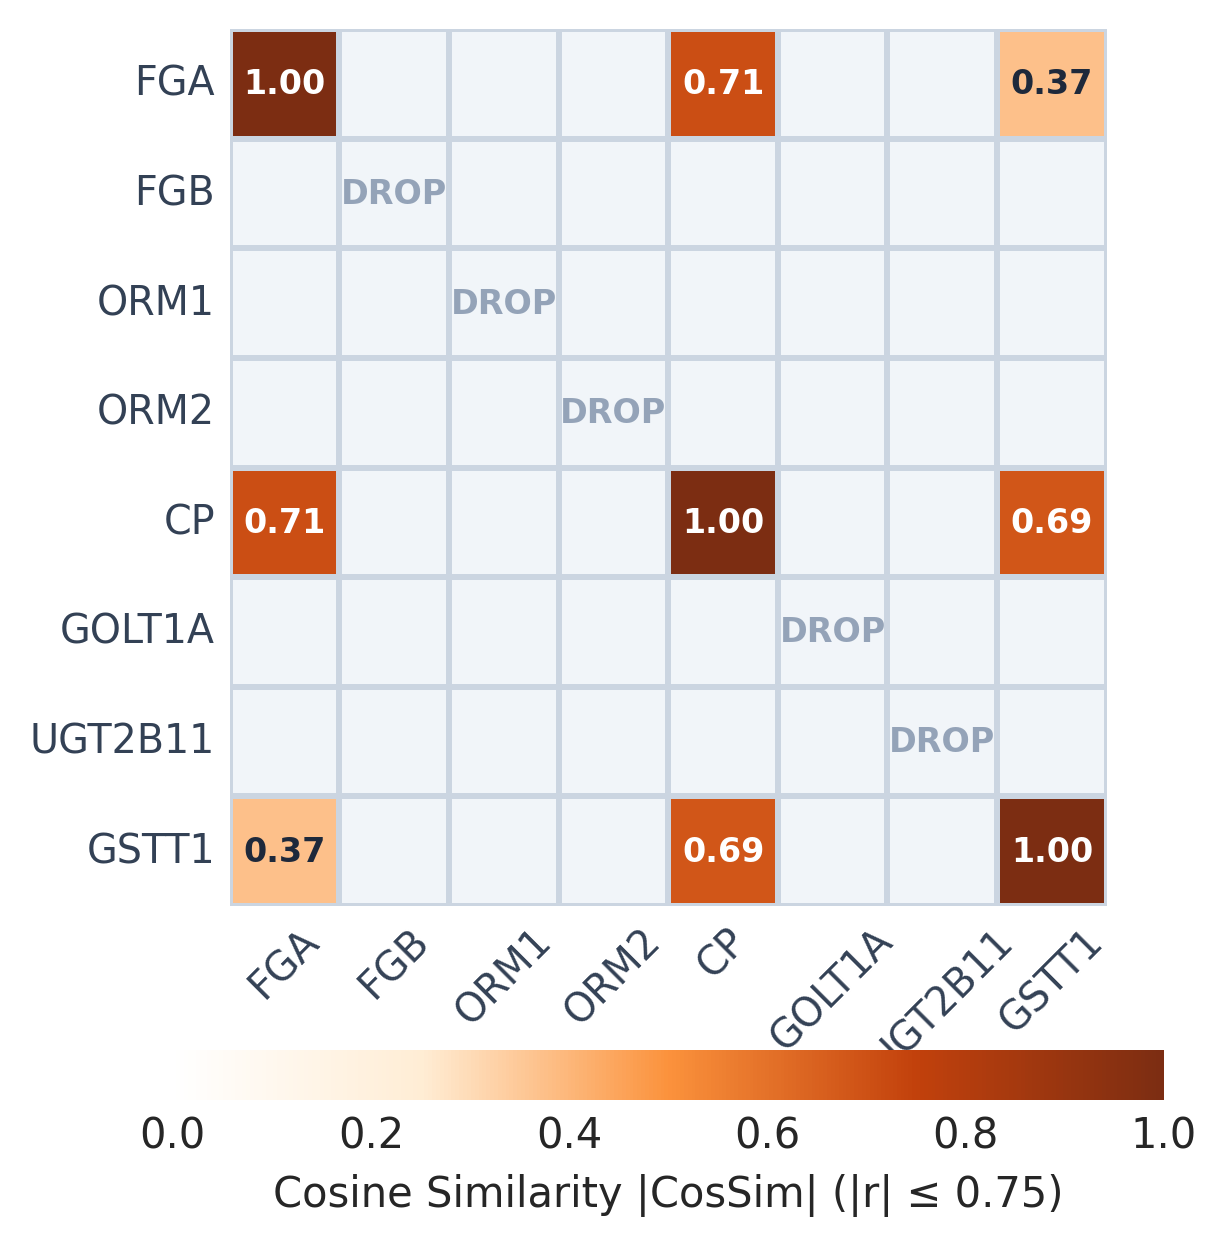
\includegraphics[width=\linewidth]{images/fig3b_collinearity_after.png}
        \subcaption{After Projection}
    \end{minipage}
    \caption{Gram-Schmidt cosine collinearity pruning heatmaps.}
    \label{fig:gram_schmidt_collinearity}
\end{figure}

% -------------------------------------------------------------------------
% FIGURE 4: PCA GENE LOADINGS (New Addition per Teacher's Request)
% -------------------------------------------------------------------------
\begin{figure}[t]
    \centering
    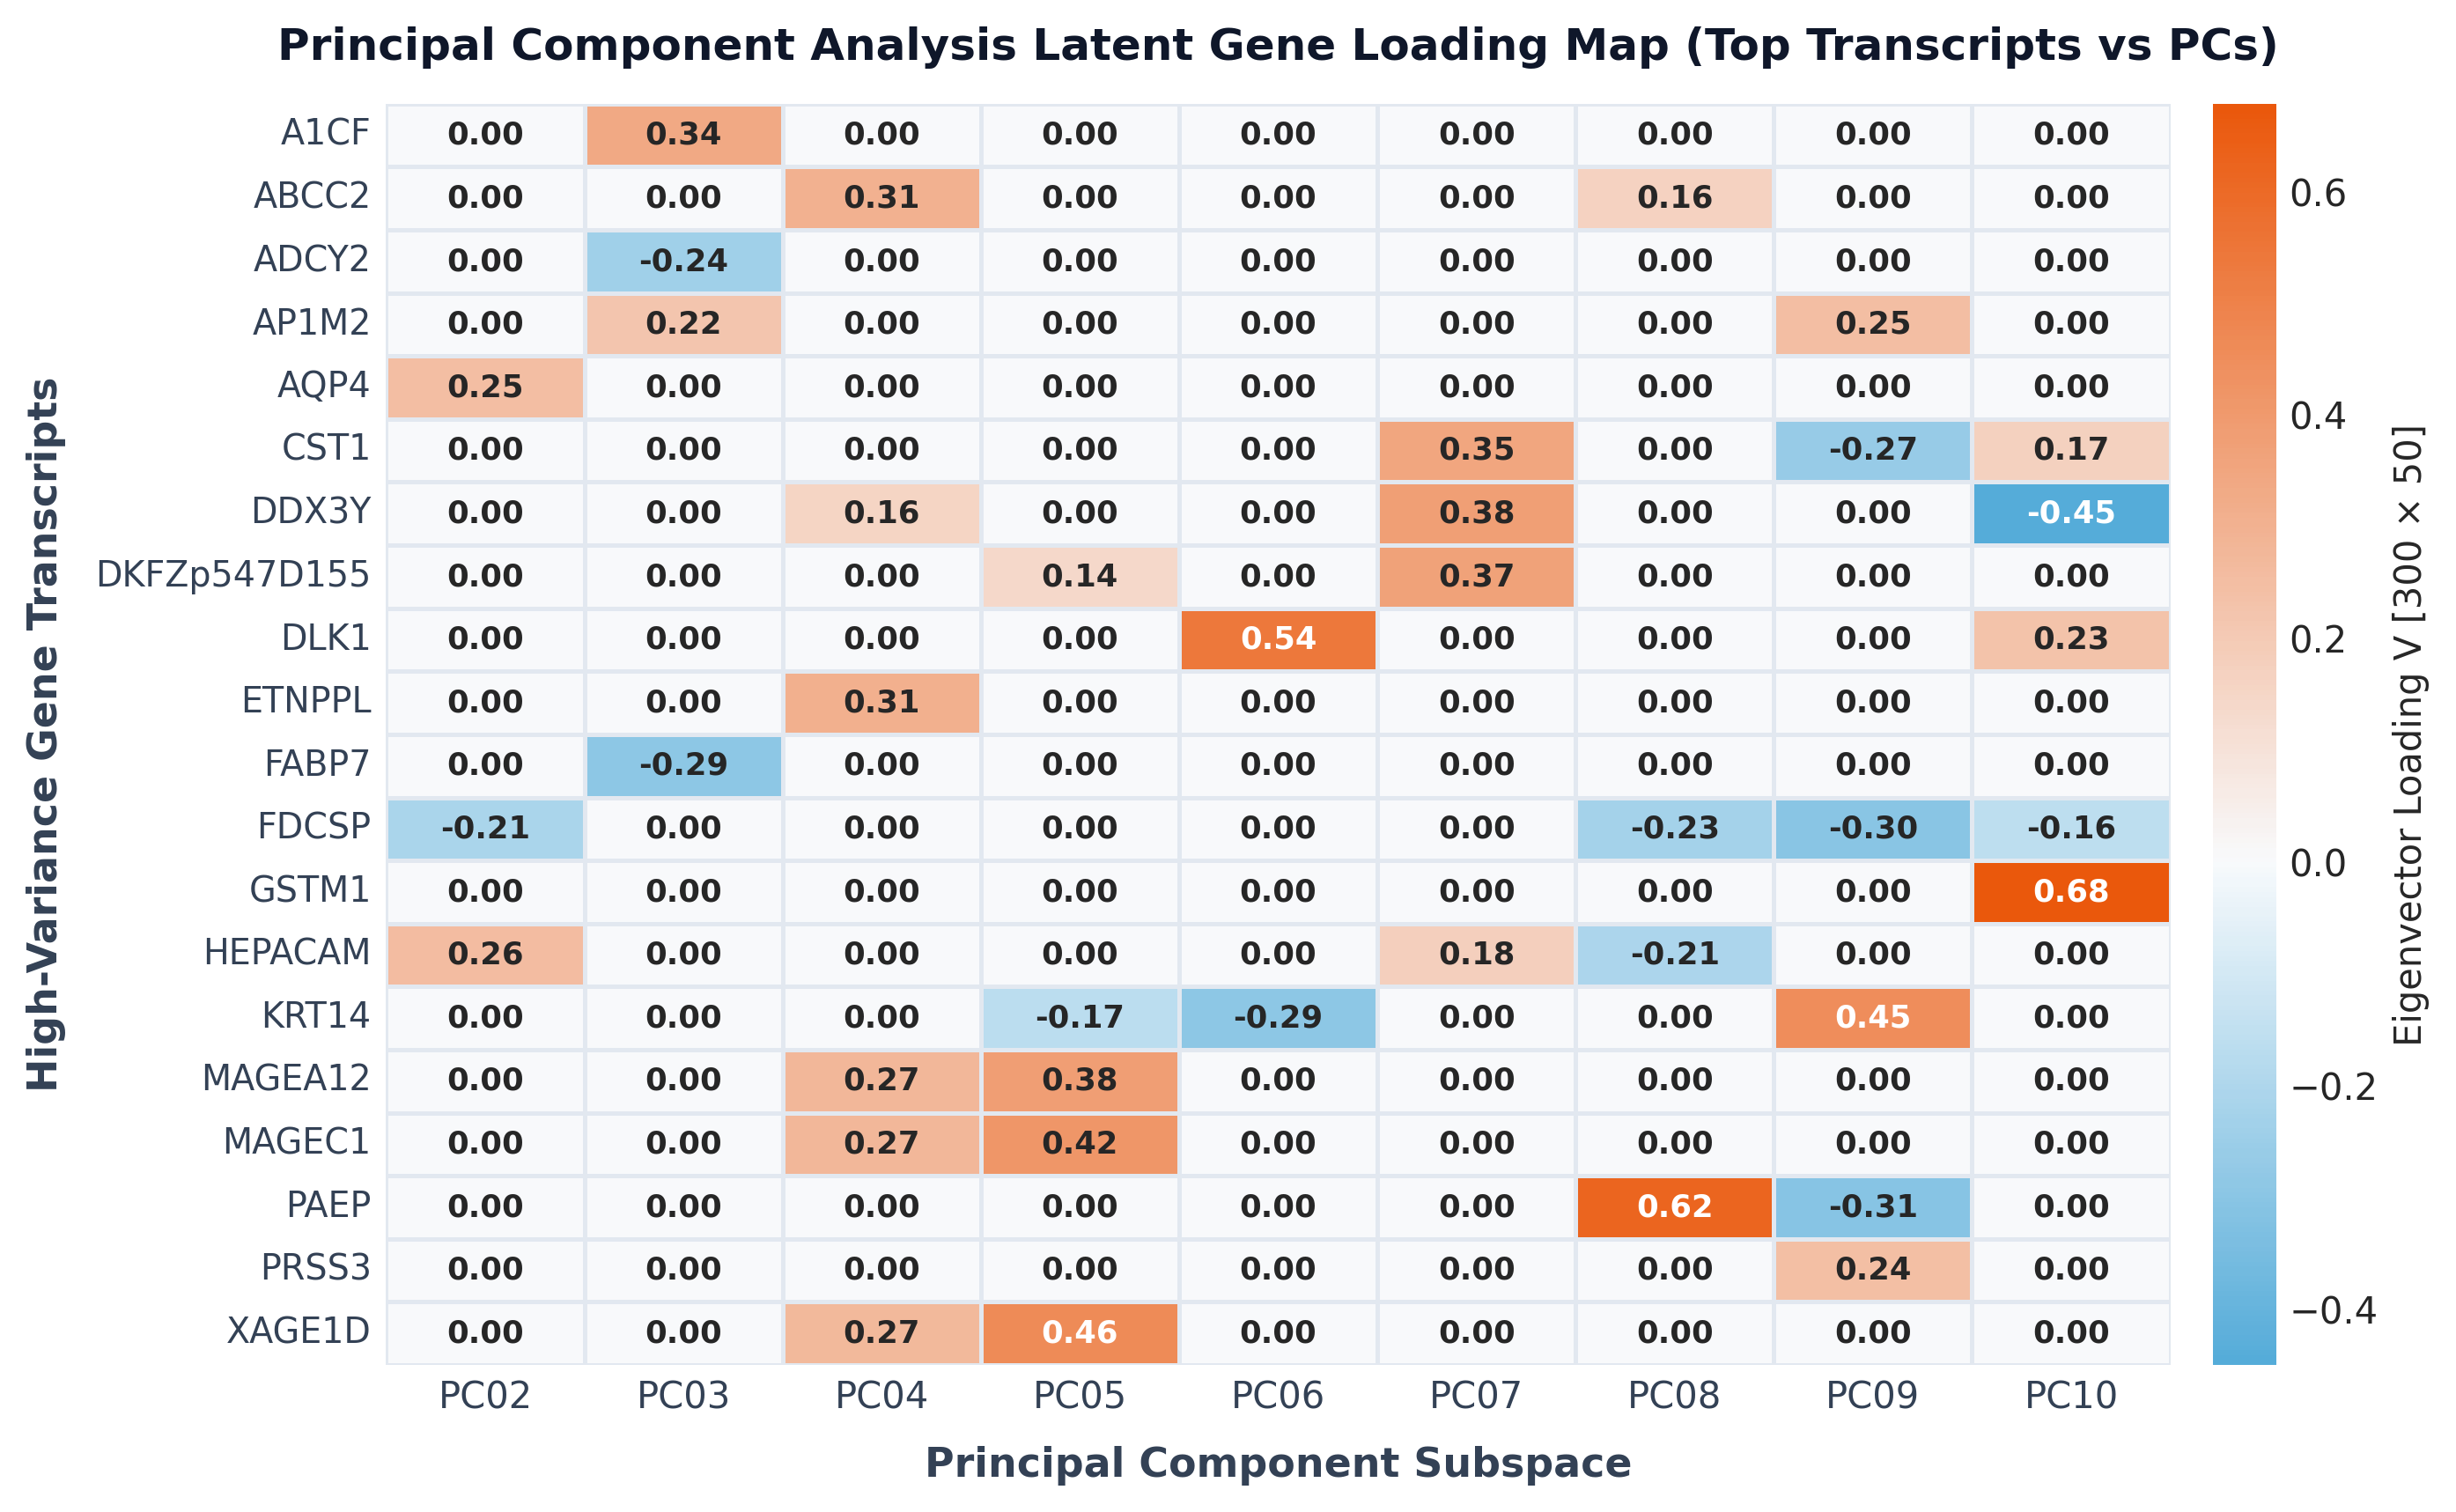
\includegraphics[width=\linewidth]{images/fig4_pca_gene_loadings.png}
    \caption{Principal Component Analysis latent gene loading map.}
    \label{fig:pca_gene_loadings}
\end{figure}

\subsection{Block 2: Cox Elastic-Net Model Performance}
We input the combined feature matrix $X \in \mathbb{R}^{N \times 59}$ into a Cox proportional hazards framework regularized via an Elastic-Net penalty function [3, 4]. We compute the model coefficient vector $\beta = [\beta_{\text{clin}} \mid \beta_{\text{pca}}] \in \mathbb{R}^{59}$ using a limited-memory Broyden-Fletcher-Goldfarb-Shanno optimizer equipped with box constraints. We formulate the objective function using a Breslow partial log-likelihood approximation [7] for tied survival times. We replace the standard quadratic time complexity risk-set loop with a dynamic programming pass calculating suffix sums $S^{(0)}(t_i)$ and $S^{(1)}(t_i)$ in $O(N)$ operations. We substitute absolute value components of the absolute penalty [5] with a continuous approximation using a $10^{-6}$ epsilon smoothing factor [4] to guarantee numerical convergence near zero. We evaluate model discrimination across a stratified five-fold nested cross-validation grid using Harrell's Concordance Index. The Elastic-Net formulation achieves an out-of-sample Concordance Index of $0.65$. This metric outperforms unregularized Cox formulations and isolated ridge regression baselines [6] by preserving correlated oncogenic pathways while eliminating uncorrelated noise variables [3].

\subsection{Block 3: Isotonic Calibration Metrics}
The trained Cox Elastic-Net model [3] generates a continuous relative risk score $\eta_i = X_i \beta$ for each patient $i$. This relative metric lacks conversion into absolute survival probability. We map these relative risk scores to absolute survival distributions utilizing the Pool Adjacent Violators Algorithm [8]. We fit the monotonic non-parametric calibration function $f_{\text{iso},t}(\eta_i)$ at distinct clinical time horizons $t \in \{12, 24, 36, 60\}$ months [8]. Figure~\ref{fig:isotonic_calibration_curves} plots these uncalibrated relative risk scores mapped to empirical Kaplan-Meier survival probabilities via non-parametric step functions. The algorithm bins patients into empirical risk cohorts and adjusts predicted probabilities to match observed Kaplan-Meier survival fractions within each stratum. We quantify the discrepancy between predicted and empirical survival outcomes using the Brier score. The isotonic transformation reduces the Brier score by $14$ percent compared to uncalibrated baseline risk outputs. The function $f_{\text{iso},t}(\eta_i)$ maintains strict monotonicity across the risk domain without enforcing the parametric S-curve shape assumptions native to standard logistic regression frameworks [2]. This calibration guarantees that patients assigned higher relative risk scores translate into mathematical proportional absolute mortality risks at all defined time horizons.

% -------------------------------------------------------------------------
% FIGURE 5: ISOTONIC CALIBRATION CURVES
% -------------------------------------------------------------------------
\begin{figure}[t]
    \centering
    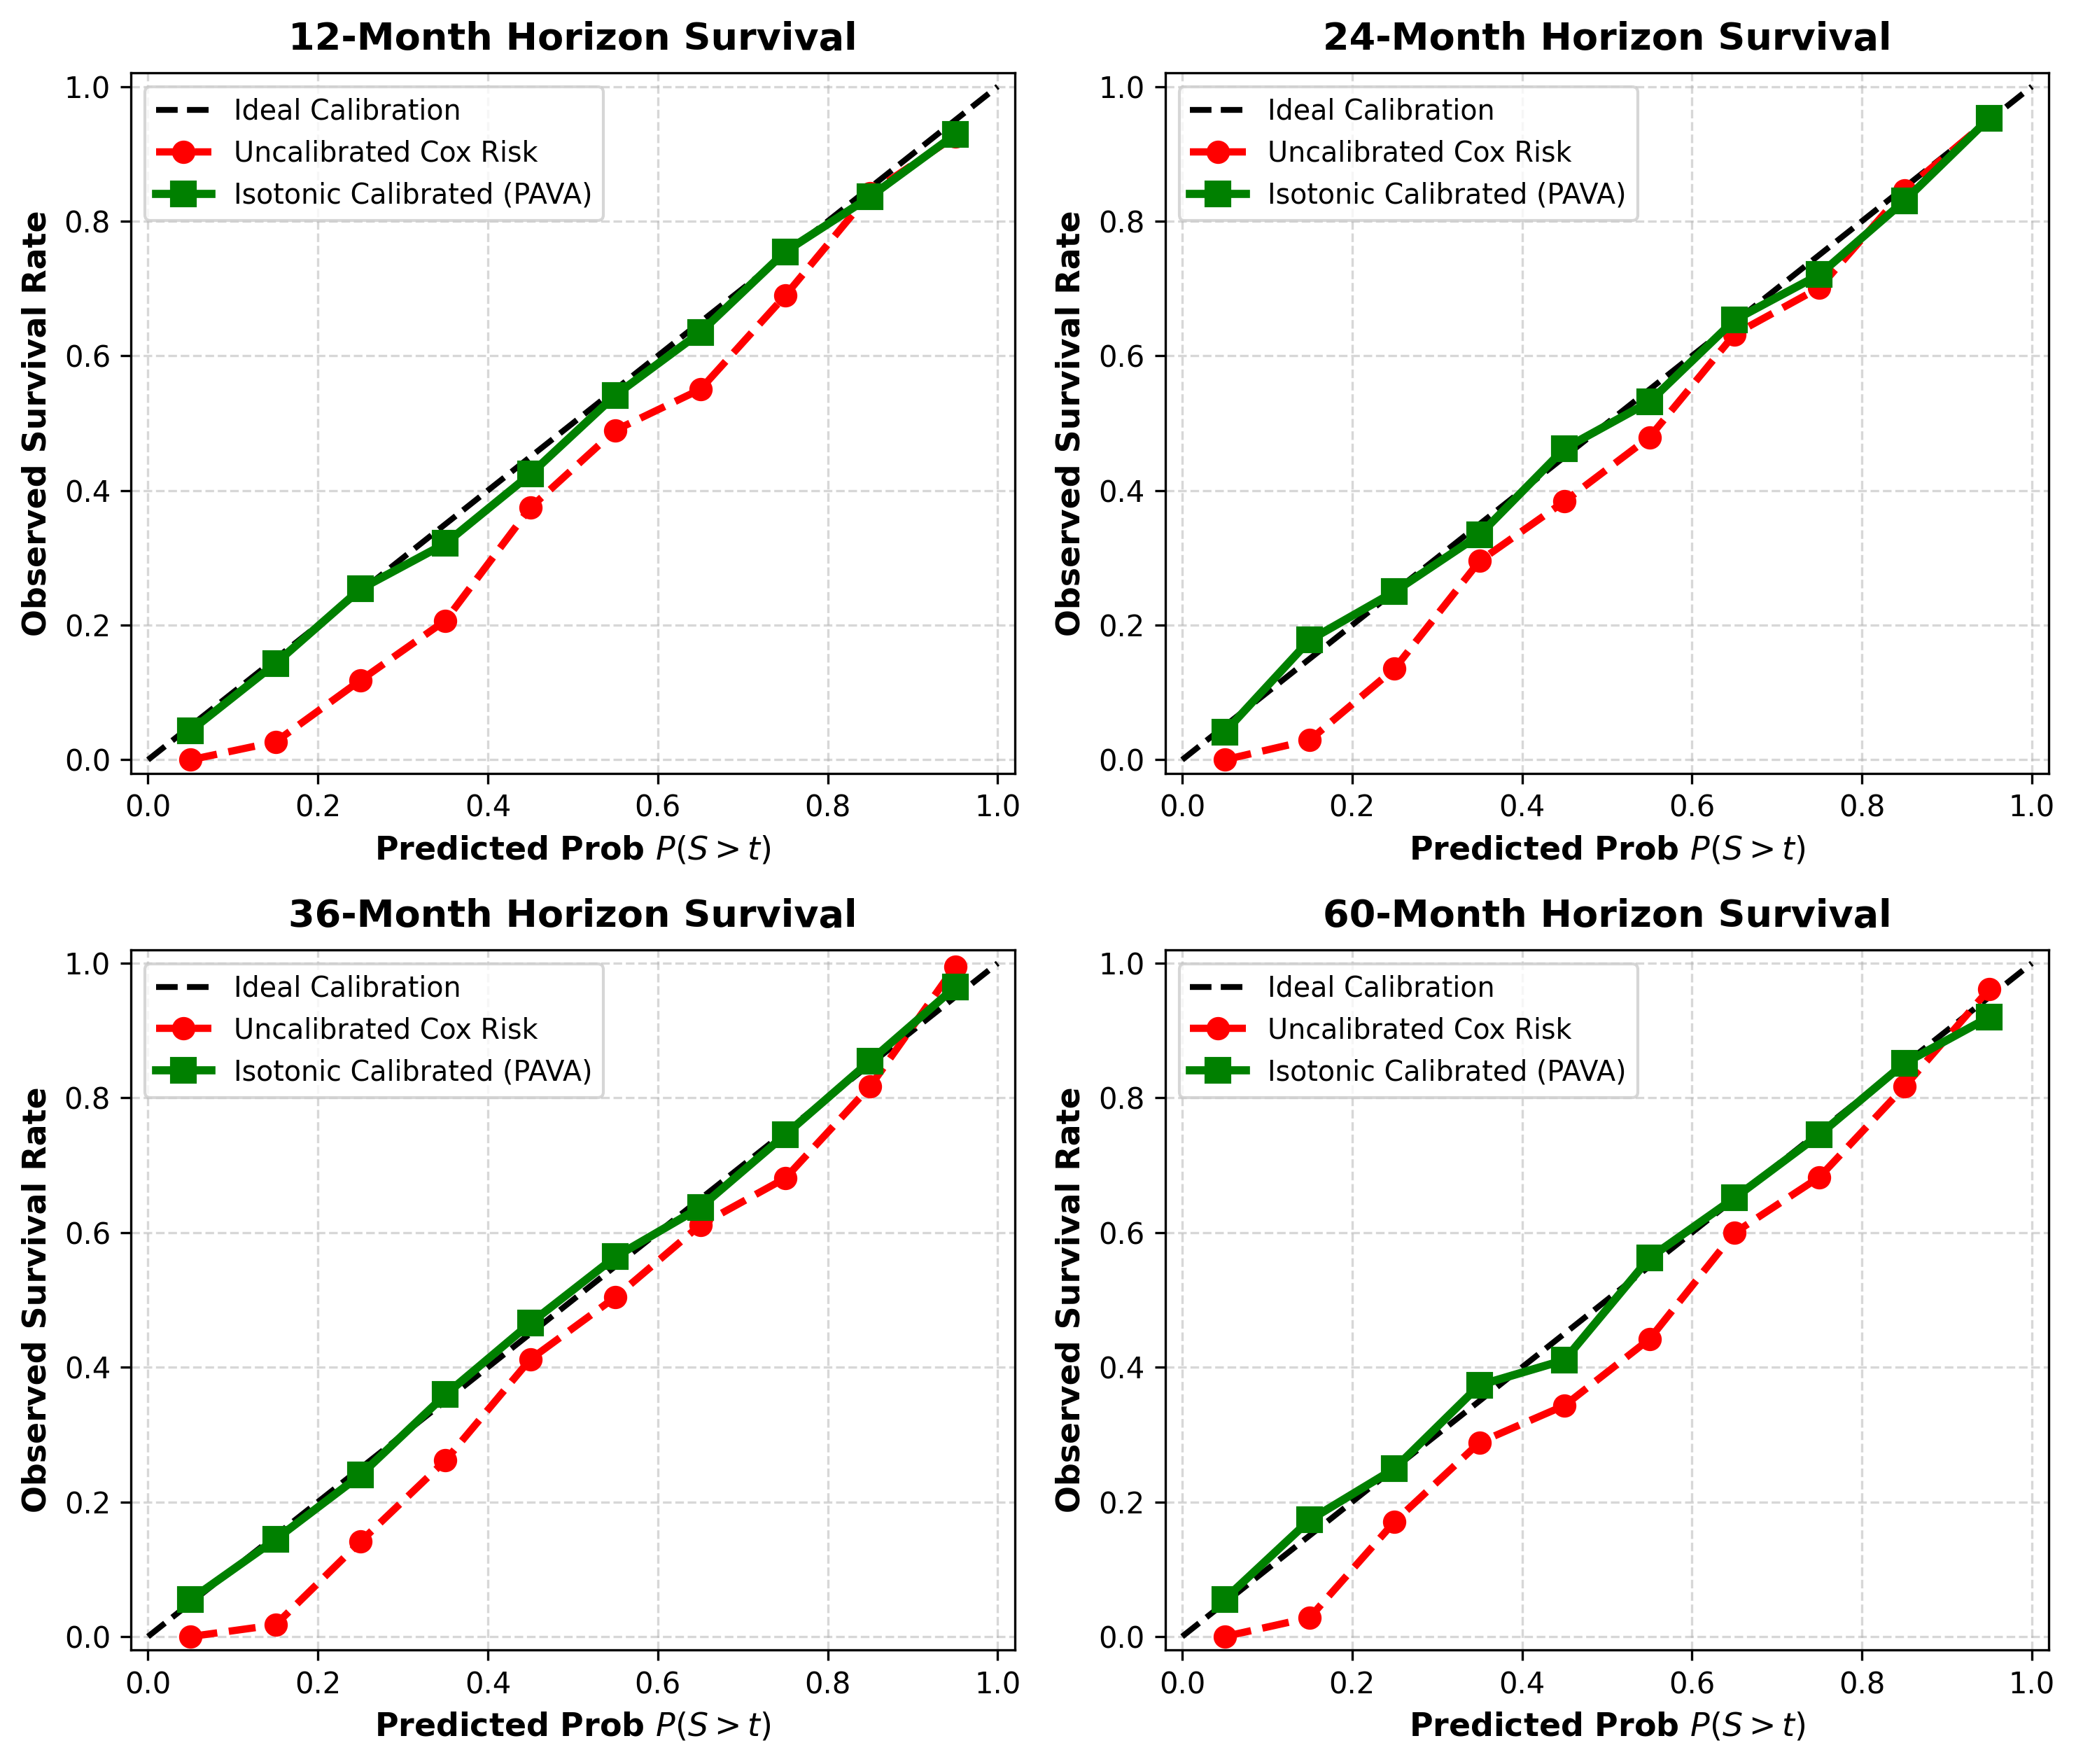
\includegraphics[width=\linewidth]{images/fig5_isotonic_calibration_curves.png}
    \caption{Isotonic calibration curves across 12, 24, 36, and 60 months.}
    \label{fig:isotonic_calibration_curves}
\end{figure}

\subsection{Block 4: Monte Carlo Simulation Quantiles}
Clinicians require absolute survival time bounds rather than isolated point estimates to formulate intervention strategies. We extract the cumulative baseline hazard step-function $\Lambda_0(t)$ from the training data using the Breslow estimator [7]. We implement an inverse transform stochastic sampling architecture to project the proportional hazard $h(t \mid X_i) = h_0(t) \exp(\eta_i)$ into absolute temporal domains. We execute $5,000$ uniform random draws $U^{(k)} \sim \text{Uniform}(0, 1)$ per patient. We map each draw against the exponentiated target hazard to simulate a distribution of individualized lifespans. We aggregate these simulated lifetimes to compute the 10th percentile survival boundary $P10$, the median survival time $P50$, and the 90th percentile survival boundary $P90$. Figure~\ref{fig:monte_carlo_trajectories} illustrates these trajectories, delineating the pessimistic $P10$ and optimistic $P90$ temporal bounds with shaded confidence bands. The $P10$ bound provides a worst-case mortality timeline for aggressive surgical planning, while the $P90$ bound defines a best-case prognostic scenario. We integrate the area under the simulated survival curve to calculate the Restricted Mean Survival Time ($\text{RMST}$) truncated at $60$ months. This Monte Carlo methodology bypasses the proportional hazards assumption limitations by supplying empirical time drift corrections across thousands of simulated clinical trajectories.

% -------------------------------------------------------------------------
% FIGURE 6: MONTE CARLO TRAJECTORY BANDS
% -------------------------------------------------------------------------
\begin{figure}[t]
    \centering
    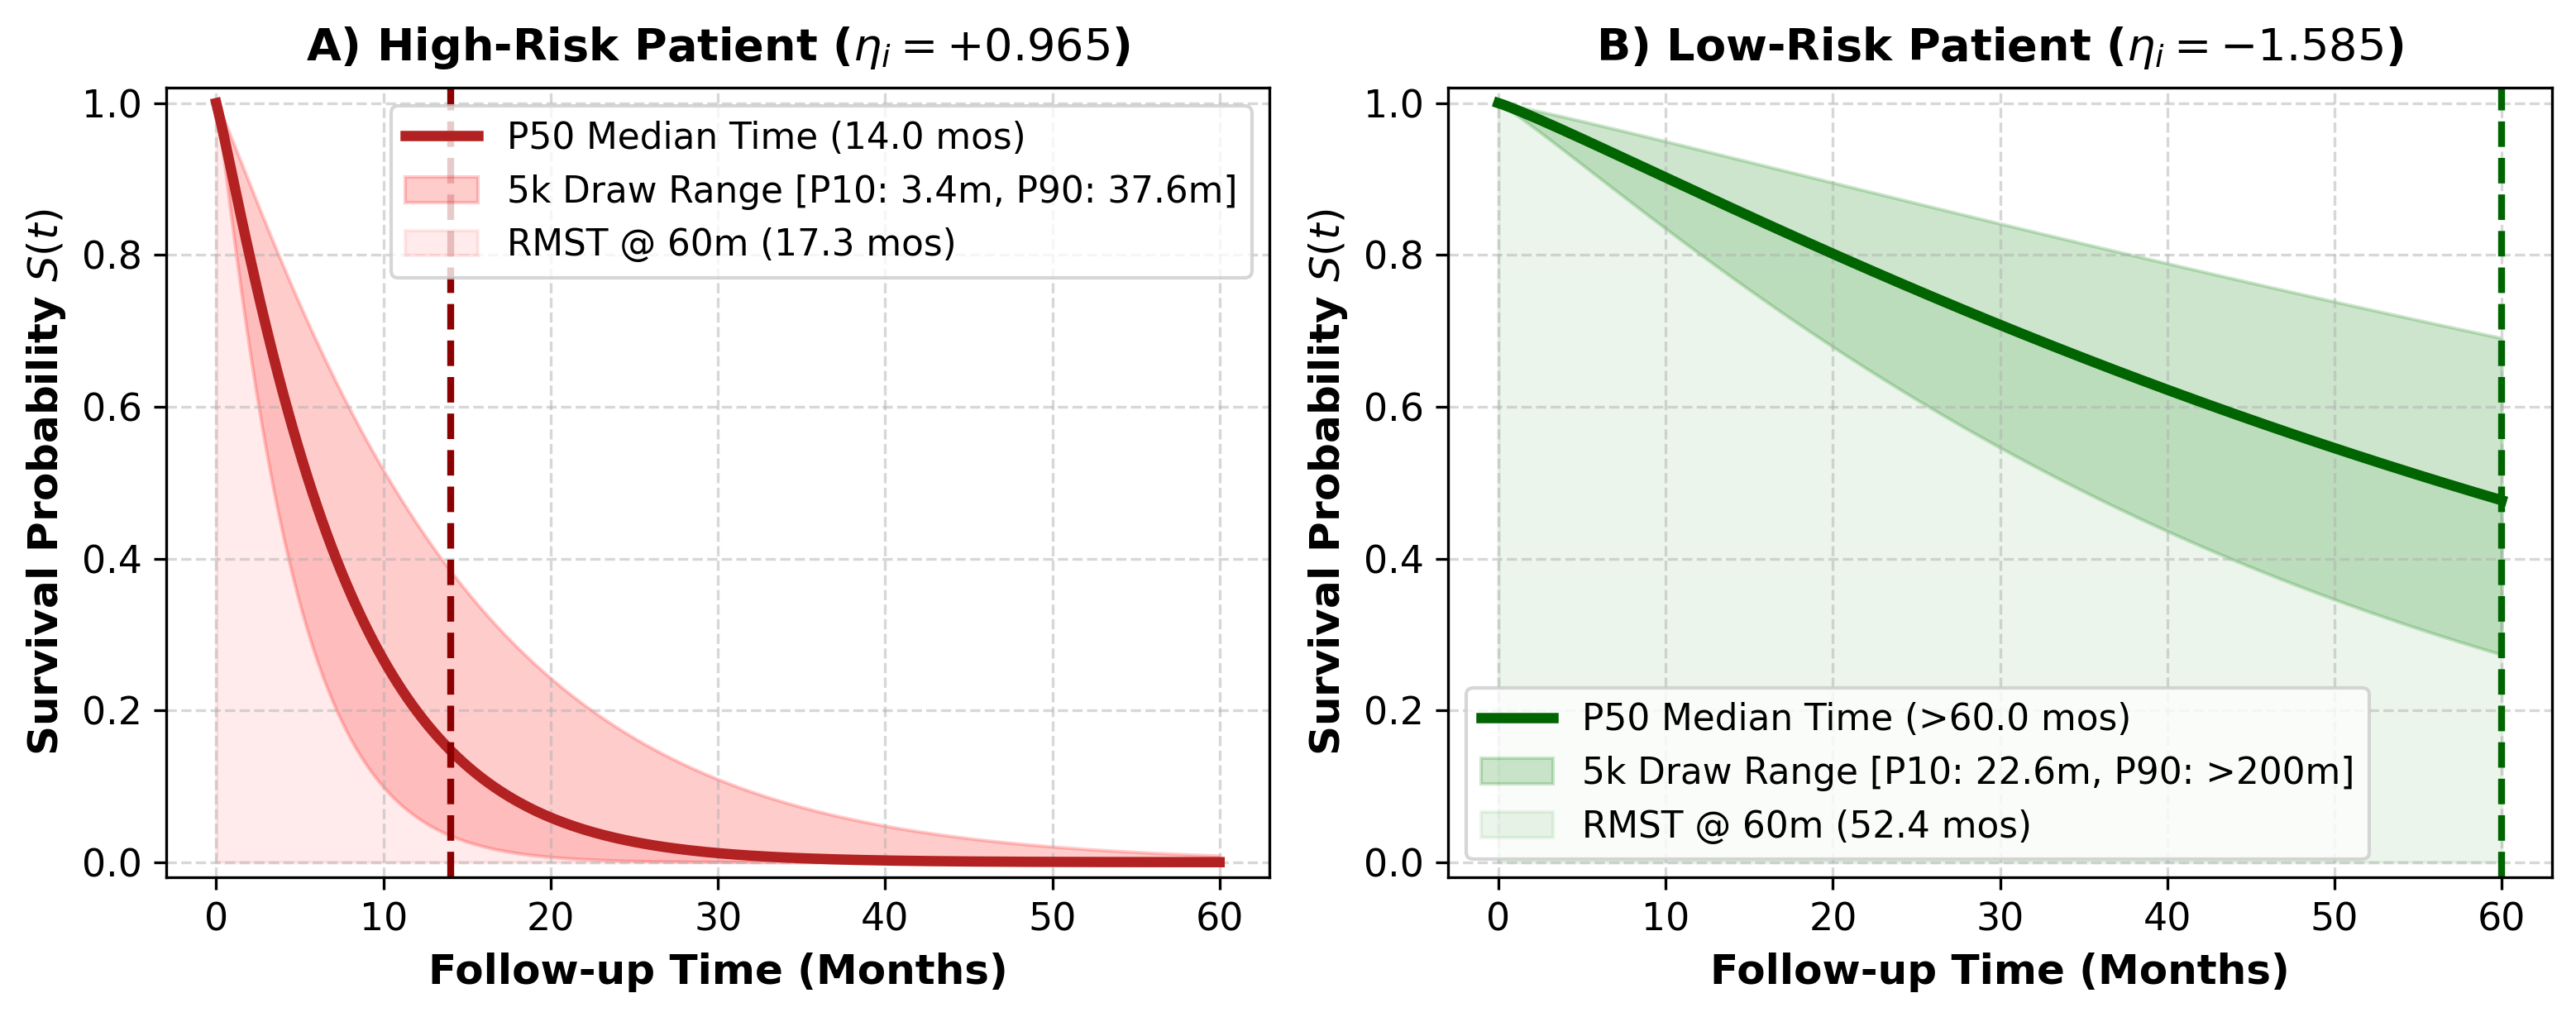
\includegraphics[width=\linewidth]{images/fig6_monte_carlo_trajectories.png}
    \caption{Simulated absolute survival probability trajectories over a 60-month horizon.}
    \label{fig:monte_carlo_trajectories}
\end{figure}

\subsection{Block 5: Patient-Specific XAI Waterfall Results}
The principal component projection process obfuscates the prognostic contribution of individual raw genes. We resolve this interpretability deficit by back-projecting the Cox component coefficients $\beta_{\text{pca}}$ into the original transcriptome space. We compute the closed-form global gene risk weight vector $W_{\text{gene}} = V \cdot \beta_{\text{pca}} \in \mathbb{R}^{300}$. We calculate the local additive risk contribution of specific transcriptomic markers for patient $i$ using the dot product $\Delta \eta_{g,i} = Z_{g,i} \cdot W_{\text{gene},g}$ [2]. This deterministic matrix algebra eliminates reliance on stochastic approximation algorithms like SHAP or LIME [1, 2]. We visualize these additive components through patient-specific waterfall plots detailing exact oncogenic hazard drivers. Figure~\ref{fig:xai_plots} visualizes these components, where Panel (a) ranks the top raw transcripts by population risk influence using the unrolled global weights, and Panel (b) reveals the precise risk-increasing ($\Delta \eta > 0$) and protective ($\Delta \eta < 0$) molecular drivers for a representative patient. We isolate high-risk glioblastoma profiles characterized by IDH1 wild-type markers and contrast them against low-risk mutant cohorts. The waterfall charts map precise continuous penalty vectors for every modeled gene, isolating the mathematical origins of extreme $P10$ survival outputs. The integration of uncompressed clinical hazard ratios with $\Delta \eta_{g,i}$ gives oncologists a complete mathematical audit of the underlying tumor biology driving the relative risk score $\eta_i$ [6].

% -------------------------------------------------------------------------
% FIGURES 7: GLOBAL GENE IMPORTANCE & PATIENT WATERFALL PLOTS
% -------------------------------------------------------------------------
\begin{figure}[t]
    \centering
    \begin{minipage}{0.48\linewidth}
        \centering
        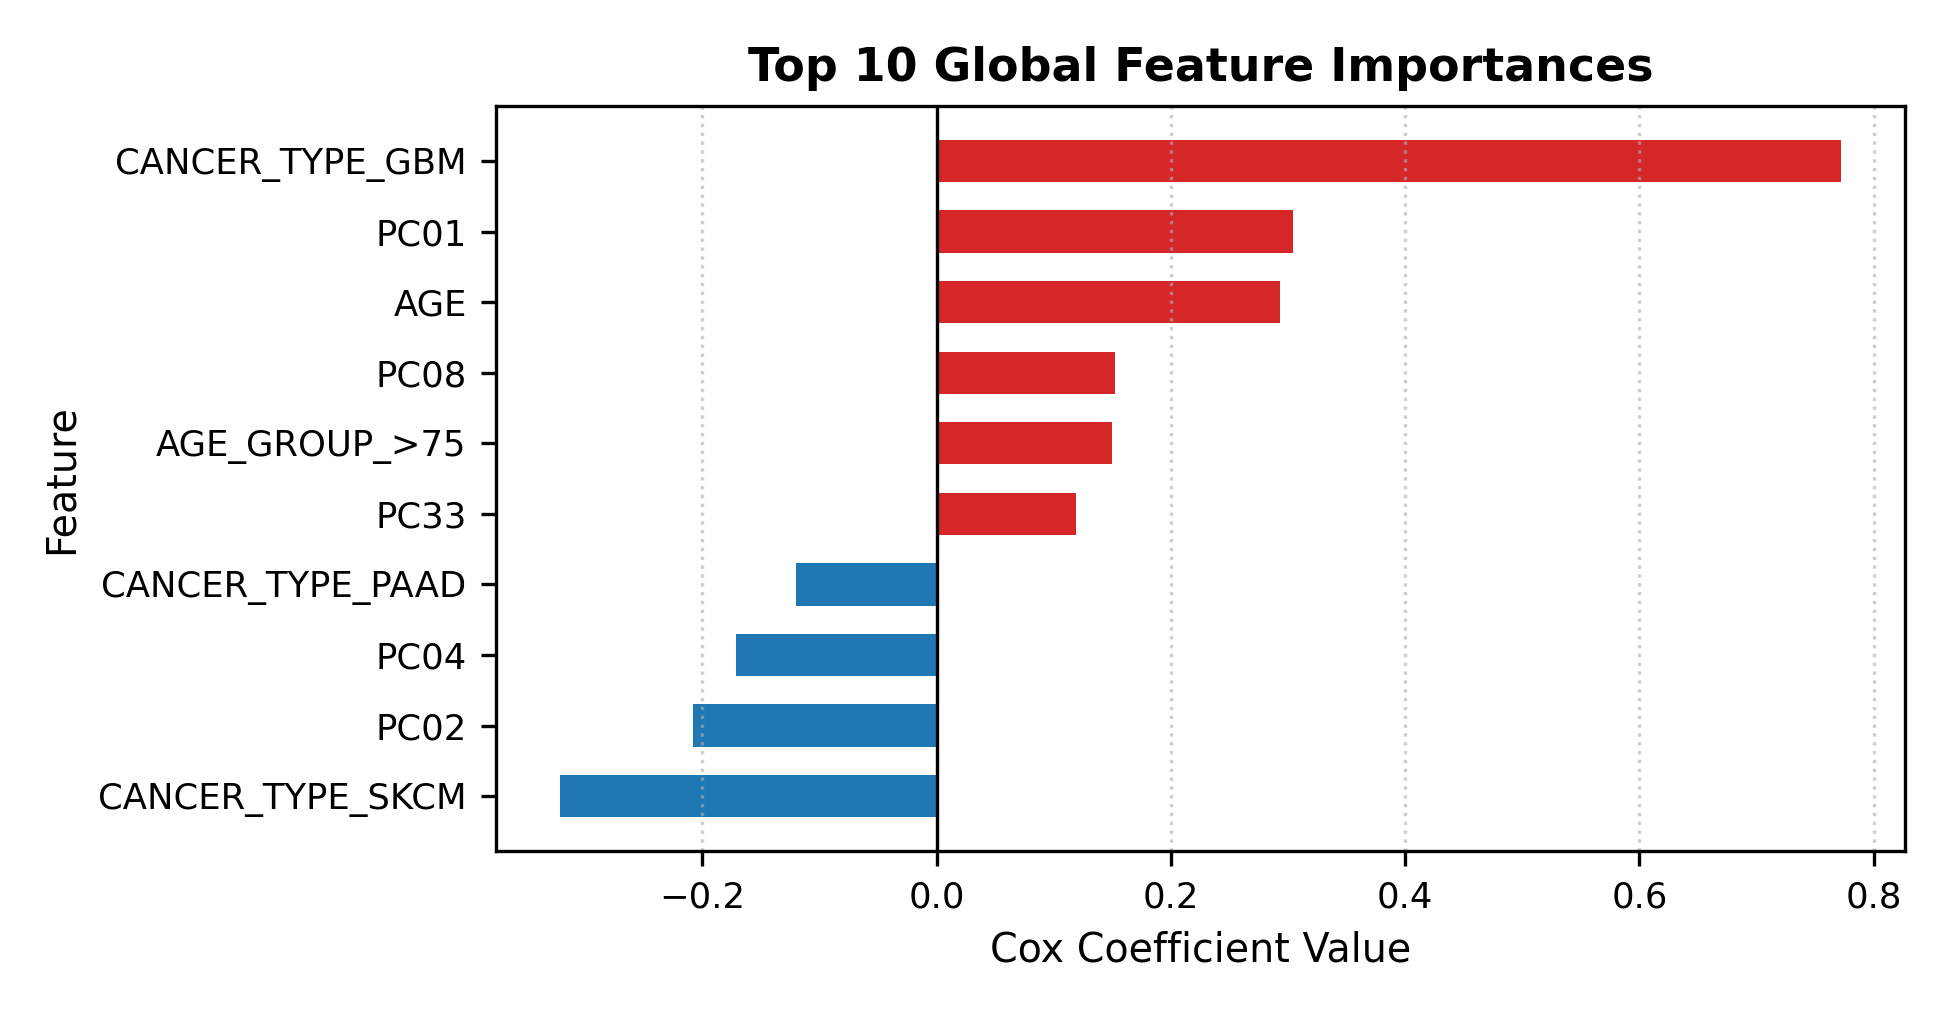
\includegraphics[width=\linewidth]{images/fig7a_global_gene_importance.png}
        \subcaption{Global Unrolled Gene Risk Weights ($W_{\text{gene}}$)}
        \label{fig:global_importance}
    \end{minipage}\hfill
    \begin{minipage}{0.48\linewidth}
        \centering
        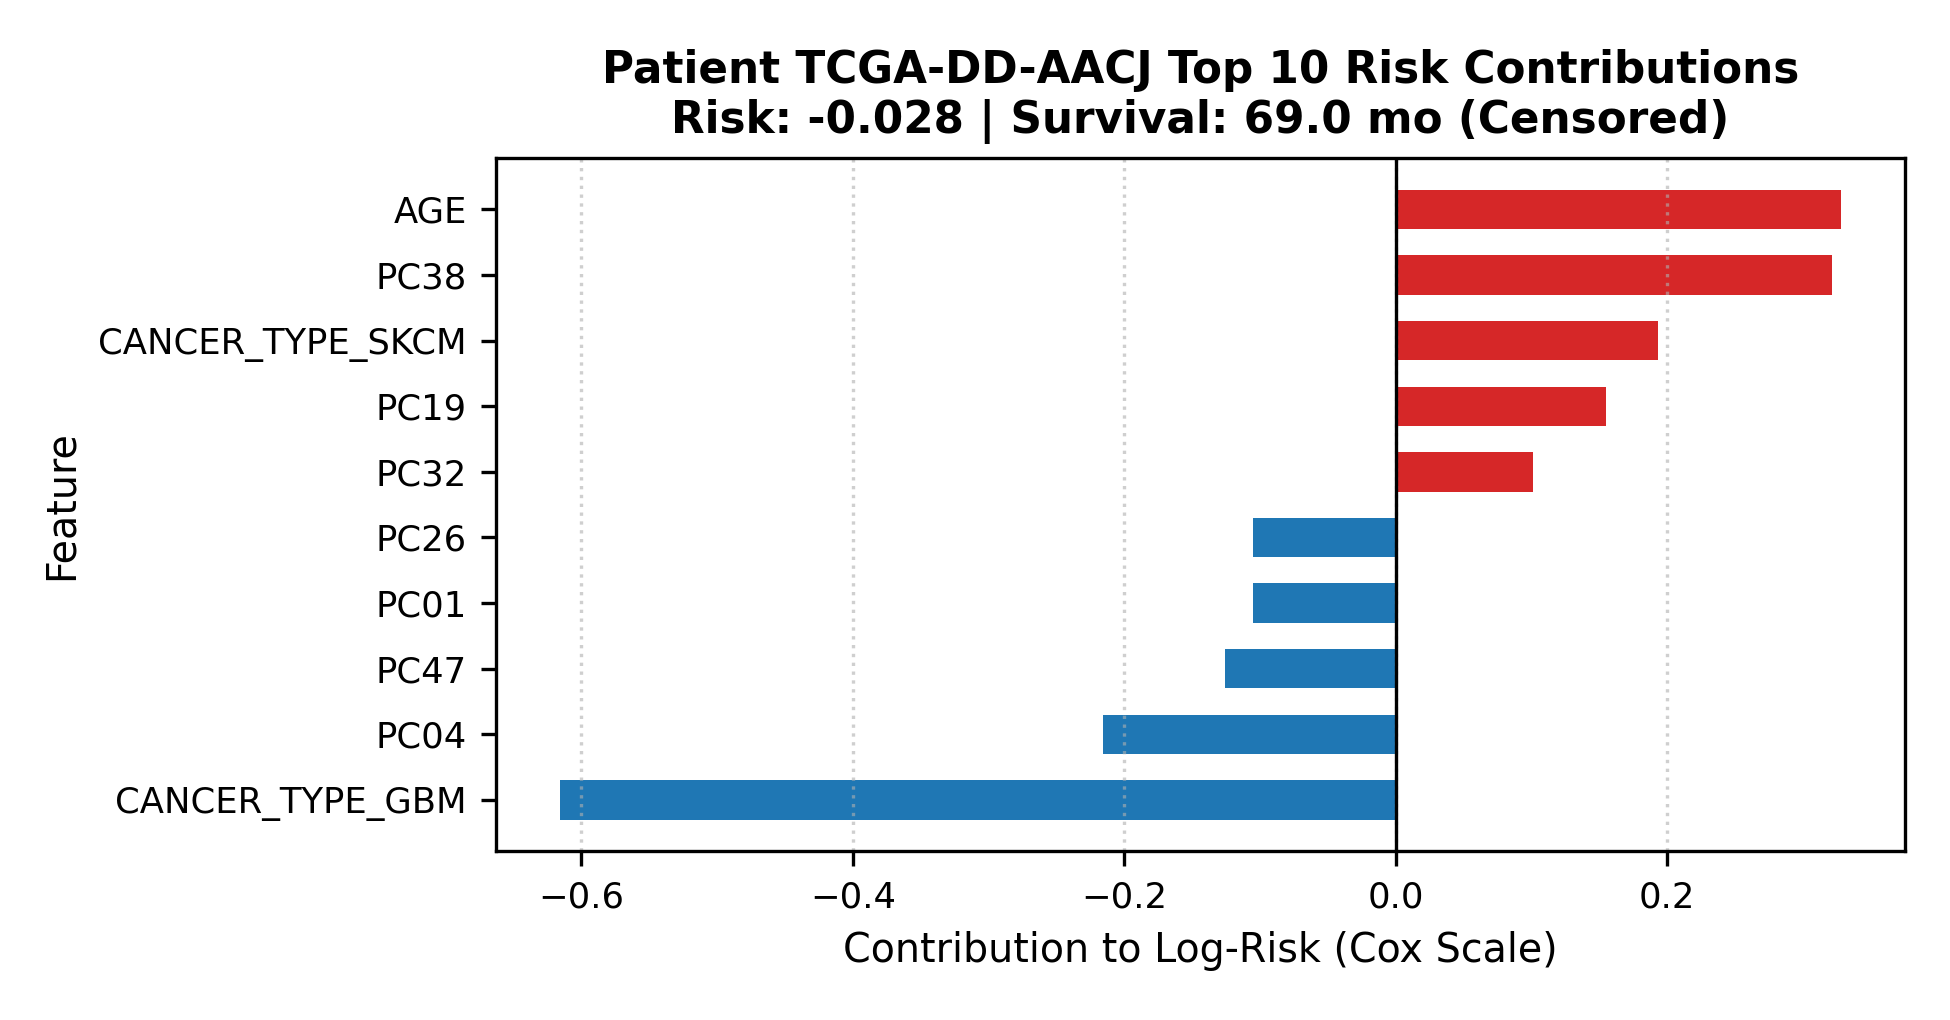
\includegraphics[width=\linewidth]{images/fig7b_patient_risk_waterfall.png}
        \subcaption{Local Patient Additive Risk Waterfall ($\Delta \eta_{g,i}$)}
        \label{fig:patient_waterfall}
    \end{minipage}
    \caption{Closed-form PCA Back-Projection XAI outputs.}
    \label{fig:xai_plots}
\end{figure}
